\documentclass[tikz,border=3mm]{standalone}
\usetikzlibrary{arrows.meta,calc,positioning}
\begin{document}
\pagecolor{white}
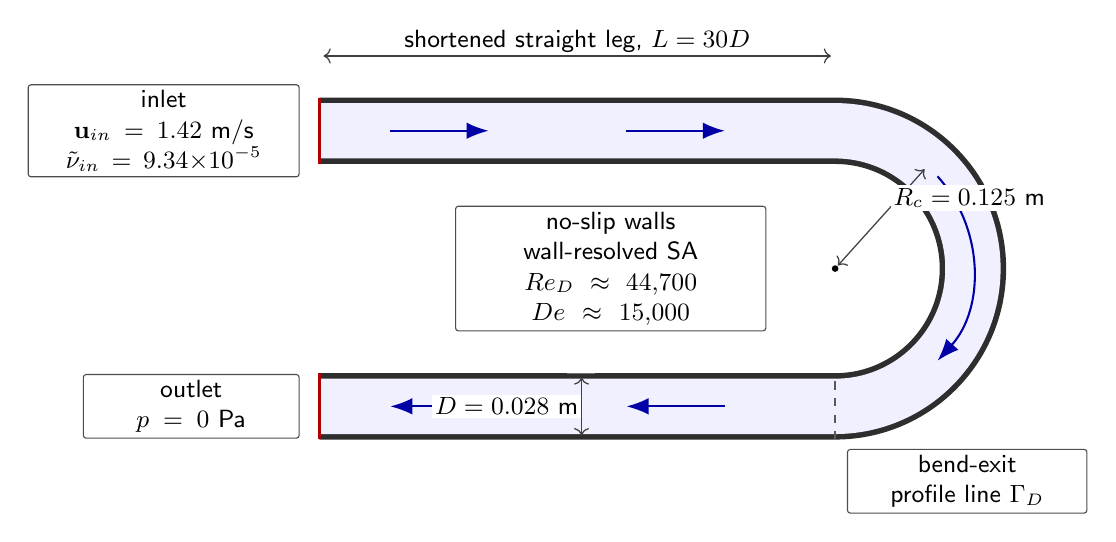
\begin{tikzpicture}[
  font=\sffamily\small,
  flow/.style={-{Latex[length=2.8mm]}, line width=0.75pt, draw=blue!65!black},
  dim/.style={<->, line width=0.45pt, draw=black!75, shorten <=1.5pt, shorten >=1.5pt},
  bc/.style={draw=black!70, fill=white, rounded corners=1pt, inner sep=2pt, align=center}
]

\def\r{1.75}
\def\cx{7.4}
\def\cy{2.75}
\def\w{0.42}
\def\xleft{0.85}
\def\ytop{\cy+\r}
\def\ybot{\cy-\r}

% Centerline path drawn as a stroked channel. The coordinate half-width \w
% matches the outer stroke, so dimension markers sit on the pipe walls.
\draw[black!82, line width=24pt, line cap=butt, line join=round]
  (\xleft,\ytop) -- (\cx,\ytop) arc[start angle=90,end angle=-90,radius=\r] -- (\xleft,\ybot);
\draw[blue!6, line width=20pt, line cap=butt, line join=round]
  (\xleft,\ytop) -- (\cx,\ytop) arc[start angle=90,end angle=-90,radius=\r] -- (\xleft,\ybot);

% Inlet and outlet planes.
\draw[red!70!black, line width=1.1pt] (\xleft,\ytop-\w) -- (\xleft,\ytop+\w);
\draw[red!70!black, line width=1.1pt] (\xleft,\ybot-\w) -- (\xleft,\ybot+\w);
\node[bc, anchor=east, text width=33mm] at (\xleft-0.25,\ytop) {inlet\\$\mathbf{u}_{in}=1.42$ m/s\\$\tilde{\nu}_{in}=9.34{\times}10^{-5}$};
\node[bc, anchor=east, text width=26mm] at (\xleft-0.25,\ybot) {outlet\\$p=0$ Pa};

% Flow arrows along the U bend.
\draw[flow] (1.75,\ytop) -- (3.00,\ytop);
\draw[flow] (4.75,\ytop) -- (6.00,\ytop);
\draw[flow] ({\cx+\r*cos(42)},{\cy+\r*sin(42)}) arc[start angle=42,end angle=-42,radius=\r];
\draw[flow] (6.00,\ybot) -- (4.75,\ybot);
\draw[flow] (3.00,\ybot) -- (1.75,\ybot);

% Radius of curvature, drawn on top of the channel with a clear label.
\coordinate (bendcenter) at (\cx,\cy);
\coordinate (radiuspoint) at ({\cx+\r*cos(48)},{\cy+\r*sin(48)});
\draw[dim] (bendcenter) -- (radiuspoint);
\node[fill=white, inner sep=1pt, anchor=south west] at ($(bendcenter)!0.53!(radiuspoint)+(0.08,0.04)$) {$R_c=0.125$ m};
\fill[black] (bendcenter) circle (1.2pt);

% Pipe diameter. Arrowheads are shortened so they remain inside the pipe walls.
\draw[black!55, line width=0.4pt] (4.00,\ybot-\w) -- (4.35,\ybot-\w);
\draw[black!55, line width=0.4pt] (4.00,\ybot+\w) -- (4.35,\ybot+\w);
\draw[dim] (4.18,\ybot-\w) -- node[left, fill=white, inner sep=1pt] {$D=0.028$ m} (4.18,\ybot+\w);

% Extraction line at the start of the outlet straight section.
\draw[black!65, dashed, line width=0.8pt] (\cx,\ybot-\w) -- (\cx,\ybot+\w);
\node[bc, anchor=north west, text width=29mm] at (\cx+0.15,\ybot-\w-0.12) {bend-exit\\profile line $\Gamma_D$};

\draw[dim] (\xleft,\ytop+0.95) -- node[above, fill=white, inner sep=1pt] {shortened straight leg, $L=30D$} (\cx,\ytop+0.95);
\node[bc, text width=38mm] at (4.55,\cy) {no-slip walls\\wall-resolved SA\\$Re_D\approx44{,}700$\\$De\approx15{,}000$};

\end{tikzpicture}
\end{document}
